\begin{figure}[H]
  \centering
  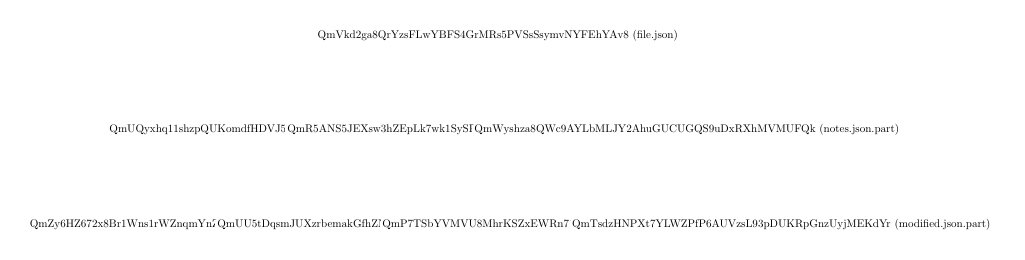
\begin{tikzpicture}[scale = 0.6, every node/.style={scale = 0.4}, every node/.append style={fill = white, rounded corners = 2pt, inner sep = 2pt, align = center}]

  \node at (0, 0) { QmVkd2ga8QrYzsFLwYBFS4GrMRs5PVSsSsymvNYFEhYAv8 (file.json) };
  
  \node at (-4, -2) { QmUQyxhq11shzpQUKomdfHDVJ5HGkrWZRFiPTLsc9hxK83 (doctor.json.part) };
  \node at (0, -2) { QmR5ANS5JEXsw3hZEpLk7wk1SySRDNnvBEdUu8RKgAybMz (metadata.json.part) };
  \node at (4, -2) { QmWyshza8QWc9AYLbMLJY2AhuGUCUGQS9uDxRXhMVMUFQk (notes.json.part) };
  
  \node at (-6, -4) { QmZy6HZ672x8Br1Wns1rWZnqmYnZ8ai1p6g5kmX2VkhDCr (id.json.part) };
  \node at (-2, -4) { QmUU5tDqsmJUXzrbemakGfhZN9edFZinA2i6iHiw3fsKim (name.json.part) };
  
  \node at (2, -4) { QmP7TSbYVMVU8MhrKSZxEWRn71F33RGSZaCPvSV47V2Anu (created.json.part) };
  \node at (6, -4) { QmTsdzHNPXt7YLWZPfP6AUVzsL93pDUKRpGnzUyjMEKdYr (modified.json.part) };

  \end{tikzpicture}
  \caption{
    Merkle tree of a JSON file
  }
  \label{fig:json_merkle_tree}
\end{figure}
